\chapter{Từ bảo toàn cục bộ đến các phương trình trường Einstein}

Các phương trình trường Einstein đủ đơn giản để viết trên một dòng và nổi tiếng là rất khó chịu khi khai triển theo các thành phần. Một metric có nhiều ký hiệu Christoffel; các ký hiệu Christoffel chứa các đạo hàm của metric; và tensor độ cong chứa cả các đạo hàm lẫn các tích của ký hiệu Christoffel. Ngay cả trước khi ta thử giải bất cứ thứ gì, phép tính cũng có thể chiếm nhiều trang. Đối với một metric cụ thể, phần mềm tính toán ký hiệu thường là cách hợp lý để xử lý việc theo dõi các hạng tử đó.

Các nguyên lý sáng sủa hơn phép tính rất nhiều. Vì vậy, chúng ta sẽ không bắt đầu bằng cách tấn công các phương trình từng thành phần một. Chúng ta sẽ hỏi lực hấp dẫn đòi hỏi loại phương trình nào. Lập luận bắt đầu từ lý thuyết Newton, đi qua bảo toàn cục bộ, và kết thúc bằng việc tìm ra tổ hợp duy nhất của các tensor độ cong có thể một cách nhất quán bằng với dòng và mật độ của năng lượng và động lượng. Xuyên suốt chương này, ta dùng \(c=1\).

\section{Con đường hai chiều của Newton}

Hấp dẫn có hai chỉ dẫn bổ sung cho nhau. Trường hấp dẫn quy định vật chất chuyển động như thế nào, còn vật chất quyết định trường hấp dẫn phải như thế nào. Con đường hai chiều này đã hiện rõ trong cơ học Newton.

Gọi \(\phi(\mathbf{x},t)\) là thế hấp dẫn Newton. Một vật thử có khối lượng \(m\) chịu lực
\begin{equation}
 \mathbf{F}=-m\nabla\phi.
\end{equation}
Kết hợp với \(\mathbf{F}=m\mathbf{a}\) làm triệt tiêu khối lượng của vật thử:
\begin{equation}
 \mathbf{a}=-\nabla\phi.
\end{equation}
Đây là chiều thứ nhất của con đường ấy. Một khi trường đã được biết, nó quy định mọi vật rơi tự do gia tốc như thế nào, không phụ thuộc vào khối lượng của vật đó.

Chiều ngược lại là phương trình Poisson,
\begin{equation}
 \nabla^2\phi=4\pi G\rho,
 \qquad
 \nabla^2=
 \frac{\partial^2}{\partial x^2}
 +\frac{\partial^2}{\partial y^2}
 +\frac{\partial^2}{\partial z^2},
 \label{eq:poisson}
\end{equation}
trong đó \(\rho(\mathbf{x},t)\) là khối lượng trên một đơn vị thể tích. Hệ số \(4\pi\) có thể được chuyển vào định nghĩa của \(G\), nhưng khi ấy nó chỉ xuất hiện trở lại ở nơi khác. Phương trình~\eqref{eq:poisson} nói rằng sự phân bố vật chất là nguồn của thế.

Đối với một vật đối xứng cầu có tổng khối lượng \(M\), nghiệm bên ngoài là
\begin{equation}
 \phi(r)=-\frac{GM}{r}.
 \label{eq:newton-potential}
\end{equation}
Mật độ có thể tập trung gần tâm, phân bố đều, hoặc giảm dần trơn tru về phía bề mặt. Nghiệm bên ngoài chỉ ghi nhận đối xứng cầu và tổng khối lượng. Bên ngoài vật chất,
\(\nabla^2\phi=0\); lấy đạo hàm \(1/r\) rồi cho ra lực nghịch đảo bình phương. Nếu ta chỉ quan tâm đến miền bên ngoài, ta có thể co nguồn lại thành một điểm và dùng cùng một biểu thức ở mọi nơi trừ tại điểm đó.

\begin{classroomqa}
\audiencequestion{Mật độ có nhất thiết phải không đổi bên trong vật đối xứng cầu rồi sau đó nhảy gián đoạn về 0 tại biên của nó không?}
\lecturerresponse{Không. Đối với lập luận này, nó phải đối xứng cầu, nhưng không cần phải không đổi và cũng không cần phải nhảy. Nó có thể giảm trơn tru về 0. Không chi tiết bên trong nào trong số đó làm thay đổi thế bên ngoài, vốn chỉ phụ thuộc vào tổng khối lượng.
\lecturetimestamp{00:09:13--00:09:37}}
\end{classroomqa}

Mô tả theo trường này trông cục bộ hơn một lực trực tiếp giữa các khối lượng ở xa, nhưng hấp dẫn Newton vẫn chứa tác dụng tức thời từ xa. Dời nguồn đi, và thế Newton thay đổi ở mọi nơi ngay lập tức. Thuyết tương đối rộng phải thay thế cả phản ứng tức thời ấy lẫn định luật lực.

\section{Một manh mối ở trường yếu, chưa phải là phương trình}

Phiên bản tương đối tính của chỉ dẫn thứ nhất đã được biết: một khi metric không-thời gian đã cho, các hạt rơi tự do đi theo các đường trắc địa của không-thời gian. Bây giờ ta cần sự thay thế tương đối tính cho phương trình Poisson, tức chỉ dẫn mà theo đó vật chất quyết định metric.

Hình học Schwarzschild cho một manh mối. Thành phần thời gian-thời gian của nó là
\begin{equation}
 g_{00}=1-\frac{2GM}{r}.
\end{equation}
Dùng phương trình~\eqref{eq:newton-potential}, ta được
\begin{equation}
 g_{00}=1+2\phi.
\end{equation}
Do đó,
\begin{equation}
 \nabla^2g_{00}=2\nabla^2\phi=8\pi G\rho.
 \label{eq:weak-mnemonic}
\end{equation}

Phương trình~\eqref{eq:weak-mnemonic} cần được hiểu một cách dè dặt. Nó là một mẹo gợi nhớ, không phải phương trình Einstein. Nó dùng một thành phần được chọn riêng của metric và một nguồn phi tương đối tính. Dù vậy, nó cho thấy đúng cấu trúc mà ta đang tìm kiếm: một mật độ vật chất ở một vế và các đạo hàm bậc hai của hình học ở vế kia. Nó là chiếc cầu thô sơ từ phương trình Poisson đến một phương trình trường hiệp biến.

Bây giờ vế phải cần được xem xét kỹ hơn. Trong đơn vị tương đối tính, khối lượng là năng lượng, vì vậy trước hết \(\rho\) nên được hiểu là một mật độ năng lượng. Nhưng một mật độ năng lượng không phải là một đối tượng tương đối tính đầy đủ. Để thấy những gì đi kèm với nó, ta bắt đầu bằng một đại lượng bảo toàn đơn giản hơn.

\section{Mật độ điện tích, dòng điện và bảo toàn cục bộ}

Gọi \(Q\) là điện tích và để \(\sigma\) biểu thị mật độ điện tích:
\begin{equation}
 \sigma=\lim_{\Delta V\to0}\frac{\Delta Q}{\Delta V}.
\end{equation}
Mật độ xét xem có bao nhiêu điện tích chiếm một thể tích không gian nhỏ tại một thời điểm. Dòng điện xét một câu hỏi khác. Hãy đặt một cửa sổ định hướng vô cùng nhỏ trong không gian và đếm lượng điện tích đi qua đó trên một đơn vị diện tích trong một đơn vị thời gian. Ba định hướng khả dĩ cho ra các thành phần dòng không gian \(J^i\).

So sánh thứ nguyên này rất gợi mở. Mật độ điện tích là điện tích chia cho ba độ dài không gian. Dòng điện là điện tích chia cho hai độ dài không gian và một khoảng thời gian. Khi \(c=1\), thời gian và độ dài có cùng đơn vị, nên mật độ và dòng điện có cùng thứ nguyên. Chúng ghép lại thành một bốn-vector:
\begin{equation}
 J^\mu=(J^0,J^1,J^2,J^3),
 \qquad J^0=\sigma.
\end{equation}

Bảo toàn điện tích không chỉ đơn thuần là mệnh đề rằng tổng điện tích trong vũ trụ giữ nguyên. Nó là cục bộ. Điện tích không thể biến mất khỏi lớp học rồi tức thời xuất hiện lại ở Alpha Centauri. Nếu nó rời một vùng, nó phải đi qua biên của vùng đó. Đối với một hộp nhỏ, độ giảm điện tích bên trong bằng thông lượng hướng ra ngoài qua các mặt của nó. Định lý Gauss cho
\begin{equation}
 \dot{\sigma}+\nabla\cdot\mathbf{J}=0,
\end{equation}
hoặc, dùng quy ước tổng,
\begin{equation}
 \partial_\mu J^\mu=0.
 \label{eq:charge-continuity}
\end{equation}
Trong tọa độ cong, phương trình tensor tương ứng được viết với đạo hàm hiệp biến:
\begin{equation}
 D_\mu J^\mu=0.
\end{equation}
Mục đích của đạo hàm hiệp biến không phải để trang trí. Nó làm cho mệnh đề này có nghĩa trong mọi hệ tọa độ.

\section{Vì sao năng lượng và động lượng cần hai chỉ số}

Bản thân điện tích là bất biến. Các quan sát viên chuyển động tương đối so với nhau đồng ý về điện tích của một electron, mặc dù họ không đồng ý về mật độ điện tích hay dòng điện. Một quan sát viên đang chuyển động thấy các thể tích bị co Lorentz và có thể thấy một luồng điện tích ở nơi quan sát viên khác thấy các điện tích đứng yên. Vì vậy, mật độ và dòng điện trộn lẫn với nhau dưới một phép đổi hệ quy chiếu, mặc dù tổng điện tích thì không.

Năng lượng và động lượng phức tạp hơn. Ngay cả tổng của chúng cũng phụ thuộc hệ quy chiếu. Một quan sát viên có thể thấy một hạt đứng yên, chỉ mang năng lượng nghỉ của nó và không có động lượng không gian. Một quan sát viên khác đi ngang qua thì thấy cả động năng lẫn động lượng. Bốn đại lượng này tạo thành bốn-vector động lượng
\begin{equation}
 P^\nu=(P^0,P^1,P^2,P^3),
 \qquad P^0=E.
\end{equation}
Mỗi thành phần \(P^\nu\) được bảo toàn cục bộ. Vì thế, mỗi thành phần đều có cả mật độ lẫn dòng. Một chỉ số nhận diện đại lượng được bảo toàn; chỉ số thứ hai nhận diện mật độ hoặc hướng của dòng.

Bắt đầu với năng lượng. Mật độ của nó là \(T^{00}\). Năng lượng cũng có thể đi qua một cửa sổ, nên \(T^{0i}\) là dòng năng lượng theo hướng \(x^i\). Bây giờ xét thành phần \(i\) của động lượng. Mật độ của nó là \(T^{i0}\), và dòng của nó theo hướng \(x^j\) là \(T^{ij}\). Theo quy ước này:
\begin{itemize}
 \item \(T^{00}\) là mật độ năng lượng;
 \item \(T^{0i}\) là thông lượng năng lượng theo hướng \(i\);
 \item \(T^{i0}\) là mật độ của thành phần \(i\) của động lượng;
 \item \(T^{ij}\) là thông lượng của động lượng \(i\) qua một mặt có pháp tuyến theo \(j\).
\end{itemize}
Khối không gian \(T^{ij}\) về sau sẽ được nhận ra là ứng suất: các phần tử đường chéo của nó bao gồm các áp suất, còn các phần tử ngoài đường chéo mô tả ứng suất trượt.

\begin{classroomqa}
\audiencequestion{Khi \(T^{m0}(x)\) được gọi là mật độ của thành phần \(m\) của động lượng, thì bản thân \(x\) có nghĩa là thành phần \(m\) của vị trí không?}
\lecturerresponse{Không. Đối số \(x\) biểu thị vị trí không-thời gian tại đó mật độ được xét; nó đại diện cho tất cả các tọa độ. Chỉ số \(m\) ghi nhãn thành phần động lượng nào đang được đếm.
\lecturetimestamp{00:41:07--00:41:27}}
\end{classroomqa}

Với mỗi \(\nu\) cố định, bảo toàn cục bộ cho một phương trình liên tục:
\begin{equation}
 D_\mu T^{\nu\mu}=0.
 \label{eq:stress-continuity}
\end{equation}
Bốn giá trị của \(\nu\) cho một phương trình cho năng lượng và ba phương trình cho động lượng. Gộp lại, các mật độ và các dòng tạo thành tensor năng lượng-động lượng.

\begin{figure}[htbp]
\centering
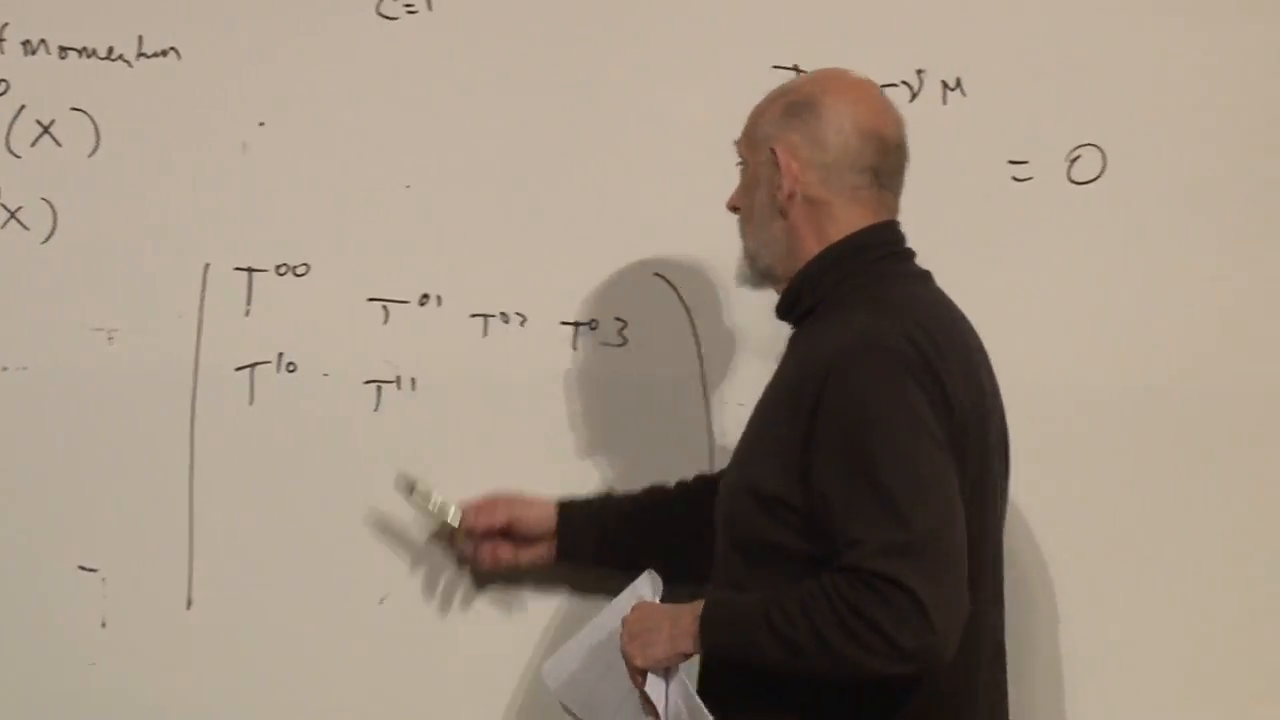
\includegraphics[width=0.84\textwidth]{lecture_09_figure_02.png}
\caption{Mảng năng lượng-động lượng đang hình thành trên bảng. Chỉ số thứ nhất chọn năng lượng hoặc một thành phần động lượng; chỉ số thứ hai chọn mật độ hoặc dòng.}
\lectureframe{00:44:30}
\end{figure}

Toàn bộ mảng là
\begin{equation}
 T^{\mu\nu}=
 \begin{pmatrix}
 T^{00}&T^{01}&T^{02}&T^{03}\\
 T^{10}&T^{11}&T^{12}&T^{13}\\
 T^{20}&T^{21}&T^{22}&T^{23}\\
 T^{30}&T^{31}&T^{32}&T^{33}
 \end{pmatrix}.
\end{equation}
Một định lý khác của cơ học tương đối tính và lý thuyết trường cho thấy tensor năng lượng-động lượng liên quan đến hấp dẫn là đối xứng:
\begin{equation}
 T^{\mu\nu}=T^{\nu\mu}.
 \label{eq:stress-symmetry}
\end{equation}
Đặc biệt, thông lượng năng lượng và mật độ động lượng là các phần tử ngoài đường chéo tương ứng khi nhìn từ hai phía đối diện. Tính đối xứng cũng cho phép ta viết phương trình~\eqref{eq:stress-continuity} dưới dạng quen thuộc
\begin{equation}
 D_\mu T^{\mu\nu}=0.
 \label{eq:stress-conservation}
\end{equation}

\begin{classroomqa}
\audiencequestion{Vì sao năng lượng-động lượng lại có thêm một chỉ số, trong khi dòng điện tích chỉ cần một chỉ số?}
\lecturerresponse{Bản thân chỉ số của dòng đã phân biệt giữa mật độ và hướng dòng. Điện tích không cần nhãn bổ sung nào vì điện tích được bảo toàn là một đại lượng vô hướng. Năng lượng và ba thành phần động lượng tự chúng đã là bốn thành phần, nên chỉ số thứ nhất cho biết đang nói tới đại lượng bảo toàn nào, còn chỉ số thứ hai cho biết đó là mật độ hay dòng.\lecturetimestamp{00:45:31--00:47:24}}
\end{classroomqa}

\begin{classroomqa}
\audiencequestion{Có phải toàn bộ ma trận \(T^{\mu\nu}\) đều đối xứng, chứ không chỉ các phần tử thông lượng năng lượng và mật độ động lượng?}
\lecturerresponse{Đúng. Toàn bộ ma trận là đối xứng. Ý nghĩa chi tiết của các phần tử không gian của nó, bao gồm áp suất và ứng suất, sẽ được phát triển sau.\lecturetimestamp{00:47:32--00:47:54}}
\end{classroomqa}

Vì vậy, mật độ năng lượng chỉ là một góc của một đối tượng lớn hơn. Nguồn của hấp dẫn không thể một cách nhất quán chỉ là \(T^{00}\); nó phải bao gồm toàn bộ tenxơ.

\section{Một định luật không thể chọn riêng một thành phần}

Nhu cầu về một phương trình tenxơ có thể thấy ra mà không cần bất kỳ phép tính độ cong nào. Giả sử \(A_i\) và \(B_i\) là các vectơ và một định luật được đề xuất chỉ nói \(A_3=B_3\). Nếu đẳng thức đó phải đúng trong mọi hệ quy chiếu quay, hãy quay trục thứ ba sang trục thứ hai. Khi đó cùng định luật ấy nói \(A_2=B_2\); một phép quay khác cho \(A_1=B_1\). Một định luật độc lập với hệ quy chiếu thực ra chính là phương trình vectơ
\begin{equation}
 A_i=B_i.
\end{equation}

Các phép biến đổi Lorentz mở rộng cùng lập luận ấy sang thời gian. Nếu \(A^0=B^0\) phải đúng trong mọi hệ quy chiếu quán tính, thì các phép boost trộn thành phần thời gian với các thành phần không gian và buộc ta có phương trình đầy đủ \(A^\mu=B^\mu\). Các định luật tương đối tính tốt phải đặt bằng nhau các tenxơ cùng loại.

Quy tắc gợi nhớ kiểu Newton đã tách riêng \(T^{00}\), nhưng phương trình tương đối tính phải có dạng
\begin{equation}
 G_{\mu\nu}=8\pi G\,T_{\mu\nu},
 \label{eq:field-schematic}
\end{equation}
trong đó ký hiệu \(G_{\mu\nu}\) lúc đầu chỉ là một chỗ giữ chỗ. Những tính chất cần có của nó nay đã rõ:
\begin{enumerate}
 \item nó phải là một tenxơ hạng hai đối xứng;
 \item nó phải được tạo từ metric, chứ không phải từ vật chất;
 \item nó nên chứa hai đạo hàm của metric;
 \item độ phân kỳ hiệp biến của nó phải bằng không.
\end{enumerate}
Điều kiện cuối cùng suy ra từ phương trình~\eqref{eq:stress-conservation}.

\section{Tìm kiếm trong các tenxơ độ cong}

Các ký hiệu Christoffel chứa một đạo hàm của metric:
\begin{equation}
 \Gamma^\sigma_{\tau\nu}
 =
 \frac12 g^{\sigma\delta}
 \left(
 \partial_\tau g_{\delta\nu}
 +\partial_\nu g_{\delta\tau}
 -\partial_\delta g_{\tau\nu}
 \right).
 \label{eq:christoffel}
\end{equation}
Chúng không phải là các tenxơ, nên tự chúng không thể cung cấp vế trái. Tenxơ độ cong Riemann là một tenxơ:
\begin{equation}
 R^\rho{}_{\sigma\mu\nu}
 =
 \partial_\mu\Gamma^\rho_{\nu\sigma}
 -\partial_\nu\Gamma^\rho_{\mu\sigma}
 +\Gamma^\rho_{\mu\lambda}\Gamma^\lambda_{\nu\sigma}
 -\Gamma^\rho_{\nu\lambda}\Gamma^\lambda_{\mu\sigma}.
 \label{eq:riemann}
\end{equation}
Hai hạng đầu của nó chứa các đạo hàm bậc hai của metric; hai hạng cuối chứa các tích của các đạo hàm bậc nhất. Đây chính là bậc vi phân mà phương trình Newton gợi ý.

Khó khăn nằm ở cấu trúc chỉ số. \(R^\rho{}_{\sigma\mu\nu}\) có bốn chỉ số, còn \(T_{\mu\nu}\) có hai. Co một cặp chỉ số trên-dưới thích hợp cho ta tenxơ Ricci,
\begin{equation}
 R_{\mu\nu}=R^\lambda{}_{\mu\lambda\nu}.
 \label{eq:ricci}
\end{equation}
Các phép co tưởng như khác hoặc triệt tiêu do các đối xứng của tenxơ Riemann, hoặc cho lại cùng một đối tượng chỉ khác bởi dấu và quy ước chỉ số. Tenxơ Ricci là đối xứng, nhưng nó chứa ít thông tin hơn tenxơ Riemann đầy đủ: nó có thể bằng không trong khi tenxơ Riemann vẫn khác không.

\begin{classroomqa}
\audiencequestion{Có thể đơn giản co hai chỉ số dưới của tenxơ Riemann không? Chẳng phải một phép co đòi hỏi một chỉ số hiệp biến và một chỉ số phản biến sao?}
\lecturerresponse{Đúng vậy. Trước hết phải nâng một chỉ số bằng metric nghịch đảo, hoặc tương đương là phép co phải bao gồm \(g^{\mu\nu}\). Viết dưới dạng \(R^\lambda{}_{\mu\lambda\nu}\) thì cặp trên-dưới cần thiết được hiện ra tường minh.\lecturetimestamp{01:00:09--01:00:33}}
\end{classroomqa}

Co tenxơ Ricci thêm một lần nữa cho ta vô hướng độ cong,
\begin{equation}
 R=g^{\mu\nu}R_{\mu\nu}.
 \label{eq:ricci-scalar}
\end{equation}
Nhân vô hướng này với \(g_{\mu\nu}\) cho ta lại một tenxơ hạng hai đối xứng khác. Vì vậy ta đã tìm được hai ứng viên tự nhiên:
\begin{equation}
 R_{\mu\nu},
 \qquad
 g_{\mu\nu}R.
\end{equation}

\begin{figure}[htbp]
\centering
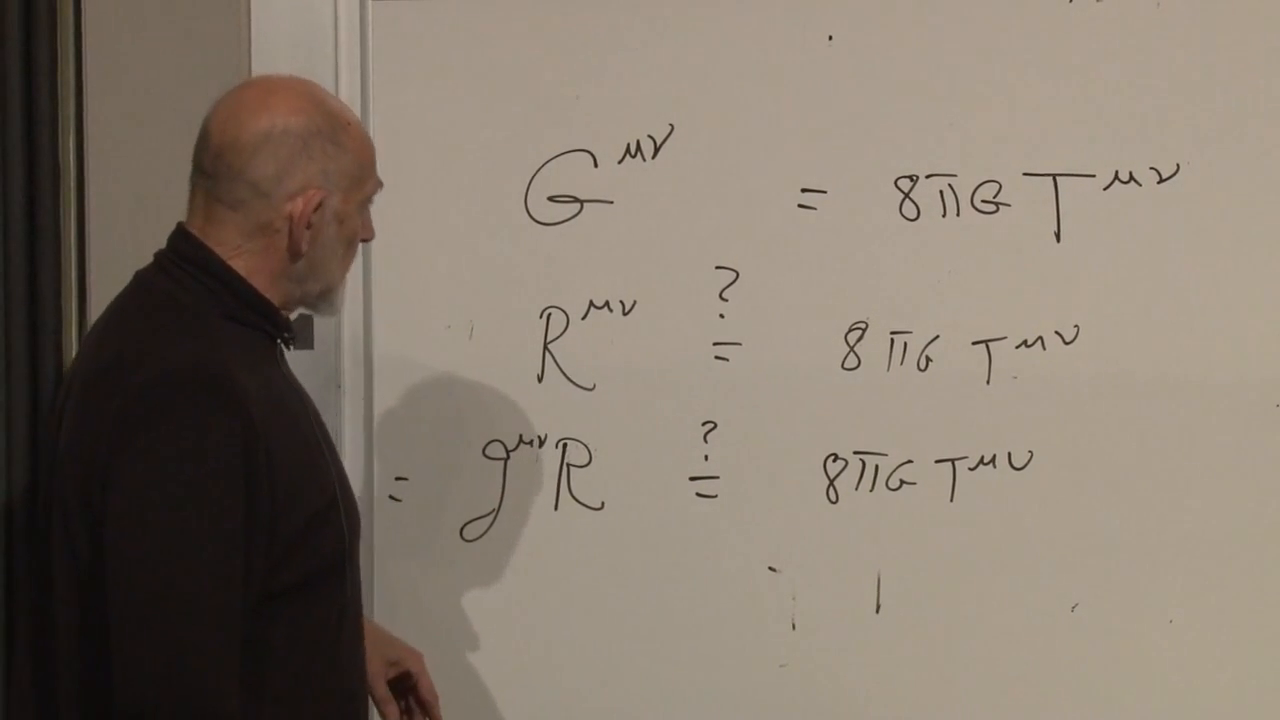
\includegraphics[width=0.78\textwidth]{lecture_09_figure_03.png}
\caption{Hai tenxơ hình học thử nghiệm trên bảng. Ở giai đoạn này cả hai đều có đúng hạng và bậc vi phân, nên mỗi cái đều đi kèm một dấu hỏi.}
\lectureframe{01:04:56}
\end{figure}

Các khả năng thăm dò là
\begin{align}
 R_{\mu\nu}&\stackrel{?}{=}8\pi G\,T_{\mu\nu},\\
 g_{\mu\nu}R&\stackrel{?}{=}8\pi G\,T_{\mu\nu}.
\end{align}
Không thể chấp nhận cái nào chỉ vì các chỉ số của nó khớp. Điều kiện bảo toàn mới là phép kiểm tra.

\section{Phép kiểm tra độ phân kỳ}

Nếu phương trình~\eqref{eq:field-schematic} là đúng, thì
\begin{equation}
 D_\mu G^{\mu\nu}=0
\end{equation}
phải suy ra như một đẳng thức đồng nhất, vì \(D_\mu T^{\mu\nu}=0\). Hãy bắt đầu với ứng viên dựa trên vô hướng độ cong. Quy tắc tích cho ta
\begin{equation}
 D_\mu\!\left(g^{\mu\nu}R\right)
 =
 \left(D_\mu g^{\mu\nu}\right)R
 +g^{\mu\nu}D_\mu R.
 \label{eq:product-rule}
\end{equation}

\begin{figure}[htbp]
\centering
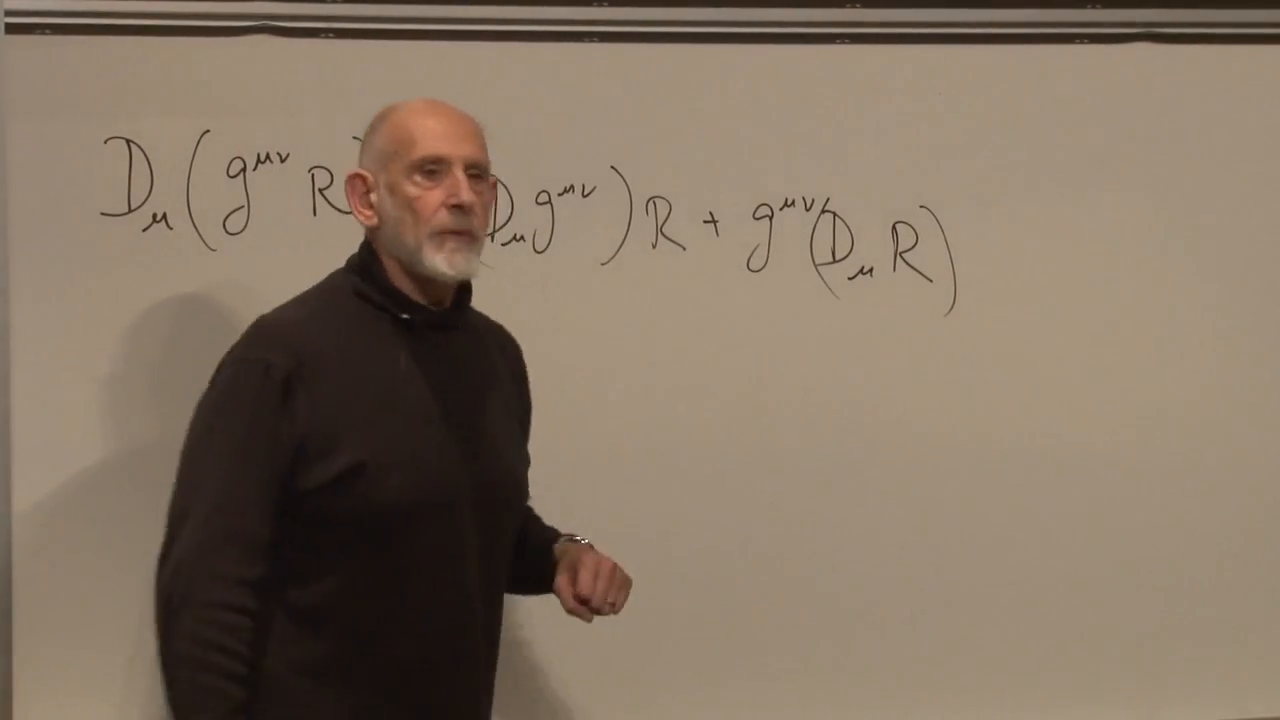
\includegraphics[width=0.84\textwidth]{lecture_09_figure_04.png}
\caption{Áp dụng quy tắc tích hiệp biến cho \(D_\mu(g^{\mu\nu}R)\).}
\lectureframe{01:07:12}
\end{figure}

Tính tương thích với metric cho biết
\begin{equation}
 D_\mu g^{\alpha\beta}=0.
 \label{eq:metric-compatibility}
\end{equation}
Đây là một tính chất hình học độc lập của liên kết Levi-Civita, không phải là hệ quả của bảo toàn năng lượng-động lượng. Vì \(R\) là một vô hướng, nên \(D_\mu R=\partial_\mu R\). Do đó phương trình~\eqref{eq:product-rule} trở thành
\begin{equation}
 D_\mu(g^{\mu\nu}R)
 =g^{\mu\nu}\partial_\mu R
 =D^\nu R,
\end{equation}
mà nói chung không bằng không. Ứng viên \(g^{\mu\nu}R\) thất bại.

Phép tính tương ứng cho tenxơ Ricci dài hơn đôi chút. Kết quả của nó là đồng nhất thức Bianchi co,
\begin{equation}
 D_\mu R^{\mu\nu}=\frac12 D^\nu R.
 \label{eq:contracted-bianchi}
\end{equation}
Vì thế \(R^{\mu\nu}\) tự nó cũng thất bại. Nhưng hai sự thất bại ấy có đúng tỉ lệ cần thiết để triệt tiêu lẫn nhau:
\begin{equation}
 D_\mu\left(
 R^{\mu\nu}-\frac12 g^{\mu\nu}R
 \right)=0.
\end{equation}
Điều này chọn ra tenxơ Einstein,
\begin{equation}
 \boxed{
 G_{\mu\nu}
 =
 R_{\mu\nu}-\frac12 g_{\mu\nu}R
 }.
 \label{eq:einstein-tensor}
\end{equation}

Trong khuôn khổ các giả thiết đang được dùng ở đây -- một tenxơ hạng hai đối xứng địa phương được tạo từ metric và chứa không quá hai đạo hàm -- tổ hợp này được xác định, ngoài một hệ số tổng thể và một hạng metric khả dĩ. Khả năng sau chính là hằng số vũ trụ, sẽ quay lại gần cuối bài giảng. Hệ số nhân với phương trình~\eqref{eq:einstein-tensor} được cố định bằng cách so khớp với hấp dẫn Newton.

\begin{classroomqa}
\audiencequestion{Có cách nào vật lý hơn để thu được phương trình trường một cách trực tiếp, thay vì thử các ứng viên rồi loại chúng bằng phương trình liên tục không?}
\lecturerresponse{Bảo toàn địa phương tự nó đã là một nguyên lý vật lý: năng lượng và động lượng không thể biến mất khỏi một vùng mà không băng qua biên của vùng đó. Cũng có một phép suy diễn cô đọng hơn từ nguyên lý tác dụng cho trường hấp dẫn. Lấy biến phân tác dụng đó cho ra cùng một phương trình, mặc dù bản thân phép tính không ngắn.\lecturetimestamp{01:17:14--01:18:41}}
\end{classroomqa}

\begin{classroomqa}
\audiencequestion{Liệu có tenxơ hình học hạng hai nào khác thỏa cùng định luật bảo toàn ấy không? Câu trả lời là mang tính vật lý hay toán học, và Einstein có biết điều đó không?}
\lecturerresponse{Dưới các giả thiết của cách xây dựng này, việc phân loại là toán học. Các đối tượng độ cong với hai đạo hàm sẵn có đều xuất phát từ tenxơ Riemann; hai ứng viên hạng hai vừa kiểm tra đã vét hết các phép co liên quan. Việc tìm ra tổ hợp không có độ phân kỳ vẫn đòi hỏi một phép tính. Các nguyên lý thì đơn giản, nhưng việc xử lý các chỉ số và dấu mới là phần công phu.\lecturetimestamp{01:18:42--01:21:44}}
\end{classroomqa}

\section{Phương trình trường và giới hạn Newton của nó}

Phương trình trường bây giờ là
\begin{equation}
 \boxed{
 R_{\mu\nu}-\frac12 g_{\mu\nu}R
 =
 8\pi G\,T_{\mu\nu}
 }.
 \label{eq:einstein-equation}
\end{equation}
Vế trái là hình học; vế phải mô tả vật chất, bức xạ và các dòng của chúng. Độ phân kỳ hiệp biến của hai vế cùng triệt tiêu.

Hệ số \(8\pi G\) không được xác định bởi lập luận về độ phân kỳ. Nó được xác định bằng cách xét một trường hấp dẫn yếu, biến thiên chậm, do vật chất chuyển động chậm gây ra, và yêu cầu thành phần thời gian-thời gian tái tạo phương trình Poisson. Trong chế độ đó \(T_{00}\simeq\rho\), còn các thành phần khác bị triệt bởi các lũy thừa của \(v/c\). Vế hình học rút về cấu trúc đạo hàm bậc hai đã được dự kiến trong phương trình~\eqref{eq:weak-mnemonic}. Sự khớp này cho chính xác chuẩn hóa trong phương trình~\eqref{eq:einstein-equation}.

Giới hạn này cũng giải thích vì sao hấp dẫn Newton dường như chỉ do mật độ khối lượng làm nguồn. Trong lý thuyết đầy đủ, mọi thành phần của \(T_{\mu\nu}\) đều gây hấp dẫn: mật độ năng lượng, dòng năng lượng, mật độ động lượng, áp suất và ứng suất cắt. Đối với vật chất phi tương đối tính thông thường, năng lượng nghỉ chiếm ưu thế. Trong vật chất tương đối tính, bức xạ, hoặc các hệ có áp suất lớn, các thành phần còn lại không thể bị bỏ qua.

Con đường lịch sử không phải là một phỏng đoán duy nhất và dễ dàng. Tenxơ Ricci trông như nỗ lực đầu tiên hiển nhiên, và hạng bổ sung \(-\tfrac12g_{\mu\nu}R\) chính là thứ khôi phục tính tương thích với bảo toàn địa phương. Một khi cấu trúc tenxơ đã được cố định, giới hạn Newton cung cấp chuẩn hóa.

\section{Phép co bỏ lại điều gì}

\begin{classroomqa}
\audiencequestion{Khi bốn chỉ số của tenxơ Riemann được co xuống còn hai, thông tin bị loại đi có mang nội dung vật lý không?}
\lecturerresponse{Có. Tenxơ Ricci không chứa toàn bộ độ cong của không-thời gian. Trường hấp dẫn không nguồn cho các ví dụ rõ nhất: tenxơ Ricci có thể bằng không trong khi độ cong thủy triều và sóng hấp dẫn vẫn còn. Phép co giữ lại phần gắn trực tiếp với phương trình nguồn cục bộ, chứ không phải mọi bậc tự do của trường hấp dẫn.\lecturetimestamp{01:21:57--01:23:10}}
\end{classroomqa}

Phép tương tự với điện từ học là hữu ích. Các phương trình Maxwell cho phép có sóng trong một vùng không chứa điện tích hay dòng điện. Tương tự, phương trình Einstein cho phép hình học không tầm thường trong một vùng mà \(T_{\mu\nu}=0\). Bây giờ ta suy ra phương trình đơn giản hơn đúng ở đó.

\section{Chân không có nghĩa là Ricci-phẳng, không phải phẳng}

Đặt
\begin{equation}
 T_{\mu\nu}=0.
\end{equation}
Khi đó Phương trình~\eqref{eq:einstein-equation} cho
\begin{equation}
 R_{\mu\nu}-\frac12g_{\mu\nu}R=0.
 \label{eq:vacuum-einstein}
\end{equation}
Lấy co với \(g^{\mu\nu}\). Vì
\begin{equation}
 g^{\mu\nu}g_{\mu\nu}
 =\delta^\mu{}_\mu=4
\end{equation}
trong bốn chiều không-thời gian, nên vết là
\begin{equation}
 R-\frac12(4)R=-R=0.
\end{equation}
Do đó
\begin{equation}
 R=0,
 \qquad
 R_{\mu\nu}=0.
 \label{eq:ricci-flat}
\end{equation}
Phương trình trường chân không là điều kiện Ricci phẳng.

Điều cốt yếu là không thay cụm từ \emph{Ricci phẳng} bằng \emph{phẳng}.
Miền ngoài Schwarzschild không chứa vật chất ở mọi nơi ngoài kỳ dị trung tâm của nó, và nó thỏa mãn \(R_{\mu\nu}=0\). Tuy vậy, tensor Riemann của nó khác không, và các lực thủy triều là có thật. Có thể kiểm tra tính Ricci phẳng bằng cách tự tính tất cả các ký hiệu Christoffel và các thành phần độ cong, dù phép tính này khá phiền phức, hoặc để một hệ đại số ký hiệu đảm nhiệm phần ghi chép tính toán. Tại kỳ dị, các biểu thức cổ điển phân kỳ; ở mọi nơi ngoài đó, phương trình chân không đều đúng.

Sóng hấp dẫn cho một ví dụ thứ hai. Chúng có thể lan truyền qua một miền không nguồn trong khi vẫn mang theo sự biến dạng không-thời gian thực sự. Do đó
\begin{equation}
 R_{\mu\nu}=0
 \quad\not\Rightarrow\quad
 R^\rho{}_{\sigma\mu\nu}=0.
\end{equation}

\section{Giữ lại nguồn: phương trình vết}

Bài giảng gần như kết thúc ở kết quả chân không, nhưng một người nghe yêu cầu lặp lại phép co mà không loại bỏ nguồn.

\begin{classroomqa}
\audiencequestion{Điều gì suy ra nếu ta thực hiện cùng phép co đó mà vẫn giữ \(T_{\mu\nu}\) trong phương trình?}
\lecturerresponse{Phép lấy vết liên hệ trực tiếp độ cong vô hướng với vết của tensor năng lượng-động lượng, và thay ngược quan hệ ấy vào sẽ cho một dạng theo tensor Ricci của phương trình trường tương đương.
\lecturetimestamp{01:29:28--01:32:20}}
\end{classroomqa}

Định nghĩa
\begin{equation}
 T=g^{\mu\nu}T_{\mu\nu}.
\end{equation}
Lấy vết của Phương trình~\eqref{eq:einstein-equation} cho
\begin{align}
 R-\frac12(4)R&=8\pi G\,T,\\
 -R&=8\pi G\,T,
\end{align}
nên
\begin{equation}
 \boxed{R=-8\pi G\,T}.
 \label{eq:trace-relation}
\end{equation}
Thay ngược vào phương trình trường thu được
\begin{equation}
 \boxed{
 R_{\mu\nu}
 =
 8\pi G
 \left(
 T_{\mu\nu}-\frac12g_{\mu\nu}T
 \right)
 }.
 \label{eq:ricci-form}
\end{equation}

\begin{figure}[htbp]
\centering
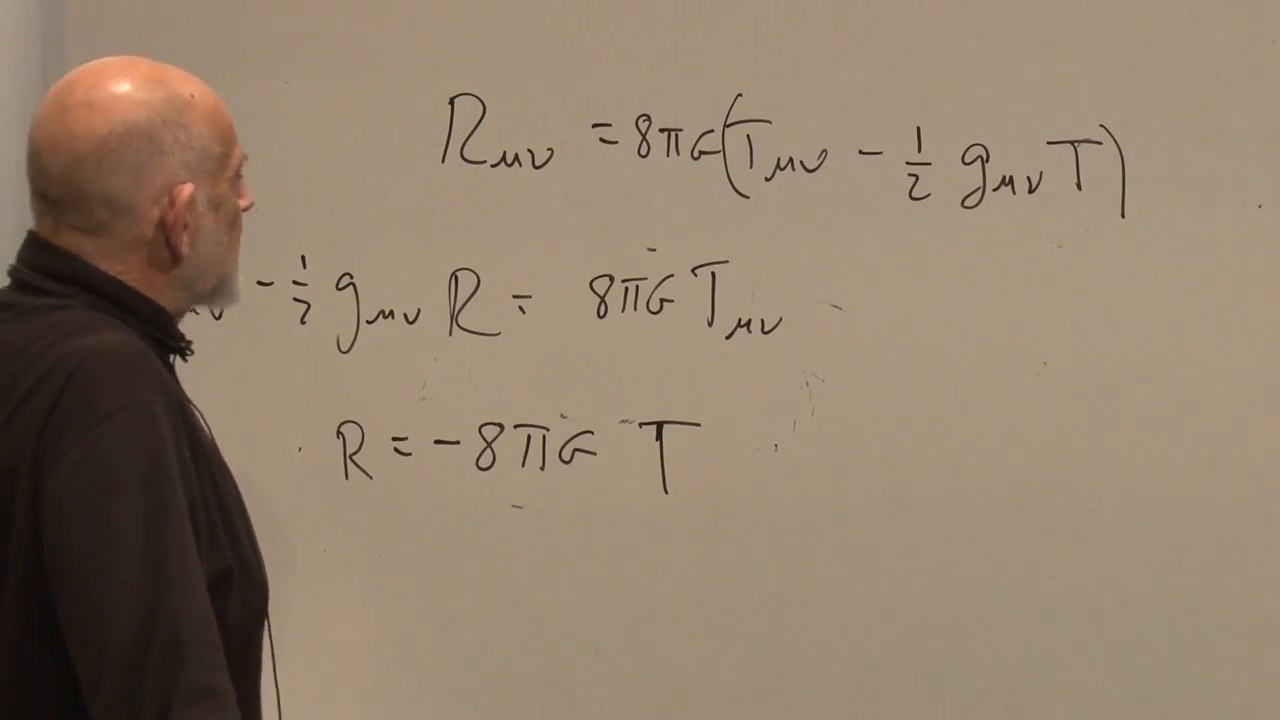
\includegraphics[width=0.82\textwidth]{lecture_09_figure_05.png}
\caption{Quan hệ vết và dạng theo tensor Ricci tương đương của phương trình Einstein.}
\lectureframe{01:32:25}
\end{figure}

\begin{classroomqa}
\audiencequestion{Đại lượng vô hướng \(T\) có ý nghĩa vật lý gì không?}
\lecturerresponse{Nó là vết của tensor năng lượng-động lượng. Đối với bức xạ điện từ, nó triệt tiêu, và điều đó cũng đúng đối với một khí lý tưởng gồm các hạt không khối lượng như photon. Vật chất có khối lượng nói chung có vết khác không. Thông qua Phương trình~\eqref{eq:trace-relation}, vết ấy xác định độ cong vô hướng.
\lecturetimestamp{01:32:20--01:33:12}}
\end{classroomqa}

\section{Ricci giữ lại bao nhiêu thông tin về độ cong?}

\begin{classroomqa}
\audiencequestion{Có một hình dung vật lý hay hình học đơn giản nào về tensor Ricci và vô hướng Ricci, có thể so sánh với phép vận chuyển song song quanh một vòng nhỏ trong trường hợp tensor Riemann, hay không?}
\lecturerresponse{Ở đây không đưa ra một hình dung nào sáng tỏ ở mức tương đương. Tensor Riemann ghi trực tiếp lại phép quay do việc vận chuyển quanh một vòng nhỏ tạo ra. Các phép co của nó đơn giản hơn về mặt đại số, nhưng ý nghĩa hình học riêng của chúng khó hình dung hơn. Tốt hơn là không dựng ra một hình dung gây hiểu lầm chỉ vì như thế sẽ tiện.
\lecturetimestamp{01:33:14--01:34:13}}
\end{classroomqa}

Lượng thông tin bị mất trong phép co phụ thuộc vào số chiều. Trong bốn chiều, tensor Riemann chứa thông tin độ cong không có trong tensor Ricci. Trong ba chiều, tensor Riemann được xác định bởi tensor Ricci. Trong hai chiều, độ cong vô hướng chứa toàn bộ thông tin độ cong độc lập. Vì vậy, hấp dẫn bốn chiều có chỗ cho các bậc tự do độ cong không nguồn không biểu lộ trong \(R_{\mu\nu}\).

\begin{classroomqa}
\audiencequestion{Nếu các tensor Riemann khác nhau có thể có cùng một tensor Ricci, thì phần thông tin bị thiếu ấy xuất hiện về mặt vật lý như thế nào?}
\lecturerresponse{Một nguồn cho trước tự nó không xác định mọi cấu hình hấp dẫn khả dĩ. Dữ liệu biên và dữ liệu ban đầu có thể bao gồm bức xạ hấp dẫn. Trong gần đúng trường yếu, ta có thể hình dung bắt đầu từ một nghiệm có nguồn rồi cộng thêm một sóng hấp dẫn tự do. Lý thuyết phi tuyến đầy đủ không cho phép chồng chập tùy ý, nhưng ví dụ ấy nhận diện đúng phần thông tin bị thiếu: độ cong lan truyền không được cố định cục bộ bởi \(T_{\mu\nu}\).
\lecturetimestamp{01:37:05--01:38:59}}
\end{classroomqa}

Hai ví dụ chân không nay khớp lại với nhau. Hình học Schwarzschild mang độ cong thủy triều ở bên ngoài một khối lượng. Một sóng hấp dẫn mang độ cong lan truyền tự do. Mỗi trường hợp đều có thể thỏa mãn \(R_{\mu\nu}=0\) mà vẫn không phẳng.

\section{Hằng số vũ trụ}

\begin{classroomqa}
\audiencequestion{Có phải không hề có thêm một hệ số chắp vá nào, chẳng hạn như hằng số vũ trụ?}
\lecturerresponse{Một hằng số vũ trụ là được phép. Nó có thể được viết ở vế hình học như một hằng số nhân với \(g_{\mu\nu}\), hoặc chuyển sang vế phải và được hiểu là một đóng góp chân không vào tensor năng lượng-động lượng. Hai cách mô tả ấy là cùng một phương trình, chỉ khác cách hạch toán các hạng.
\lecturetimestamp{01:39:01--01:40:44}}
\end{classroomqa}

Khi có hằng số vũ trụ, một quy ước thường dùng là
\begin{equation}
 G_{\mu\nu}+\Lambda g_{\mu\nu}
 =
 8\pi G\,T_{\mu\nu}.
\end{equation}
Chuyển số hạng phụ sang vế phải sẽ xác định một tensor ứng suất chân không hiệu dụng,
\begin{equation}
 T_{\mu\nu}^{(\Lambda)}
 =
 -\frac{\Lambda}{8\pi G}g_{\mu\nu}.
\end{equation}
Vì tính tương thích metric cho \(D_\mu g^{\mu\nu}=0\), số hạng phụ ấy tự động tương thích với định luật bảo toàn. Đây chính là số hạng theo metric đã được để ngỏ trong phát biểu về tính duy nhất trước đó.

\section{Sao Thủy và phép tính trường yếu}

\begin{classroomqa}
\audiencequestion{Einstein có dùng phương trình này để tính quỹ đạo của Sao Thủy không, và có thể xem cách thực hiện phép tính đó ở đâu?}
\lecturerresponse{Einstein làm việc trước khi Schwarzschild đưa ra nghiệm chính xác, nên thay vào đó ông dùng một gần đúng khoảng cách lớn đủ chính xác cho trường bên ngoài của Mặt Trời. Bán kính của Mặt Trời và quỹ đạo của Sao Thủy đều rất lớn so với bán kính Schwarzschild của Mặt Trời, nên các hiệu chỉnh tương đối tính là nhỏ. Ông có thể bắt đầu từ một quỹ đạo Kepler và tính hiệu chỉnh bằng phương pháp nhiễu loạn. Schwarzschild thu được nghiệm ngoài chính xác ngay sau đó, khiến cùng phép tính ấy trở nên có hệ thống.
\lecturetimestamp{01:40:46--01:43:48}}
\end{classroomqa}

Lý thuyết nhiễu loạn chính là như vậy: bắt đầu từ một bài toán đã giải xong, rồi tính tác động của một hiệu chỉnh nhỏ. Lực nghịch đảo bình phương của Newton tạo ra các elip Kepler khép kín. Thuyết tương đối rộng thêm vào một độ lệch nhỏ khỏi phương trình bán kính Newton, vì thế elip không khép kín sau một vòng quay; cận nhật của nó tiến lên.

Bài giảng khép lại bằng tính đặc biệt có phần kỳ lạ của các quỹ đạo lực tâm khép kín. Lực nghịch đảo bình phương là trường hợp ngoại lệ ở chỗ nó làm cho các quỹ đạo Kepler khép kín mà không tiến động. Tổng quát hơn, định lý Bertrand cũng chỉ ra dao động điều hòa đẳng hướng là thế tâm còn lại mà với nó mọi quỹ đạo liên kết đều khép kín. Hiệu chỉnh tương đối tính nhỏ phá vỡ sự suy biến Newton ấy, biến sự tiến động của Sao Thủy thành một dấu hiệu quan sát được của phương trình trường được suy ra trong chương này.